\documentclass[11pt,a4paper]{article}
\usepackage[margin=23mm]{geometry}
\usepackage{fontspec,unicode-math,booktabs,graphicx,array,hyperref}
\setmainfont{STIXGeneral}\setmathfont{STIX Two Math}\hypersetup{hidelinks}
\setlength{\parindent}{0pt}\setlength{\parskip}{5pt}
\newcommand{\tabsetup}{\small\setlength{\tabcolsep}{4pt}\renewcommand{\arraystretch}{1.10}}
\begin{document}
\begin{center}\Large\textbf{Common theories and their applications}\\[4pt]
\normalsize Nineteen topics, forty-three original manuscripts\end{center}
For each topic, $S=\sum_i c(L_i)$ is the length of the complete original
manuscripts, $U$ the length of the whole common theory, and $A=\sum_i c(A_i)$
the length of all complete applications. We report
\[
R=\frac{S}{U+A},\qquad r_i=\frac{c(L_i)}{c(A_i)}.
\]
The second comparison assumes acquisition of the whole common theory and
the declared required dependencies. Each topic pays its common theory
independently. A factor greater than one indicates a shorter written replacement.

\textbf{Complete manuscript costs.} The unit is NFC characters without
whitespace, at each topic's stated representation. Introductions, context,
proofs, companions and references remain included.
\begin{center}\tabsetup\begin{tabular}{lrrrrrr}\toprule
Topic & Originals & Sources & Common & Applications & Written & Factor\\\midrule
A & 7 & 213,803 & 49,059 & 87,019 & 136,078 & 1.571 \\
B & 5 & 124,906 & 44,905 & 69,265 & 114,170 & 1.094 \\
C & 5 & 118,433 & 30,437 & 61,248 & 91,685 & 1.292 \\
D & 3 & 47,894 & 15,632 & 29,855 & 45,487 & 1.053 \\
E & 3 & 71,375 & 19,790 & 19,513 & 39,303 & 1.816 \\
F & 2 & 69,825 & 15,876 & 27,398 & 43,274 & 1.614 \\
G & 2 & 73,199 & 30,928 & 85,207 & 116,135 & 0.630 \\
Affine & 1 & 32,767 & 19,070 & 22,638 & 41,708 & 0.786 \\
Represent. & 1 & 25,348 & 11,288 & 13,688 & 24,976 & 1.015 \\
Chamber & 2 & 35,802 & 15,199 & 21,254 & 36,453 & 0.982 \\
Matching & 1 & 37,951 & 16,732 & 17,168 & 33,900 & 1.119 \\
Chiral & 1 & 29,599 & 8,831 & 23,171 & 32,002 & 0.925 \\
Operations & 3 & 200,891 & 58,215 & 100,379 & 158,594 & 1.267 \\
Gluing & 1 & 27,081 & 28,416 & 11,565 & 39,981 & 0.677 \\
Rank contr. & 1 & 15,530 & 6,937 & 10,555 & 17,492 & 0.888 \\
Locally proj. & 2 & 26,490 & 25,498 & 11,966 & 37,464 & 0.707 \\
Mathieu & 1 & 13,736 & 5,516 & 35,862 & 41,378 & 0.332 \\
Rank augm. & 1 & 33,604 & 13,904 & 14,096 & 28,000 & 1.200 \\
Mixes & 1 & 57,753 & 12,615 & 31,077 & 43,692 & 1.322 \\
\bottomrule\end{tabular}\end{center}
\textbf{Scope.} The active catalogue contains 106 accessible originals:
43 admitted principal-result recoveries with measurements and 63 awaiting
complete recovery. The 55 unavailable originals from the historical catalogue
of 161 remain archived outside the analysis. No singleton is excluded.
An admission covers the specified principal results, corrections and retained
inputs; it does not establish every auxiliary claim or answer every conjecture.

\textbf{Representations.} B and C include complete authored-text renderings
where original PDFs are unavailable. F, Mixes, rank contraction, rank
augmentation and the Mathieu census use raw untrimmed PDFs. Other topics
retain their declared calibrated and selected text. No pooled factor is
formed across these different representations.
\newpage
\textbf{The complete common theory and every application.}
The dark bar is the sum of the original manuscript costs. Blue segments
are complete common papers; green segments are complete applications.
All companions and complete written tables remain charged.
\begin{center}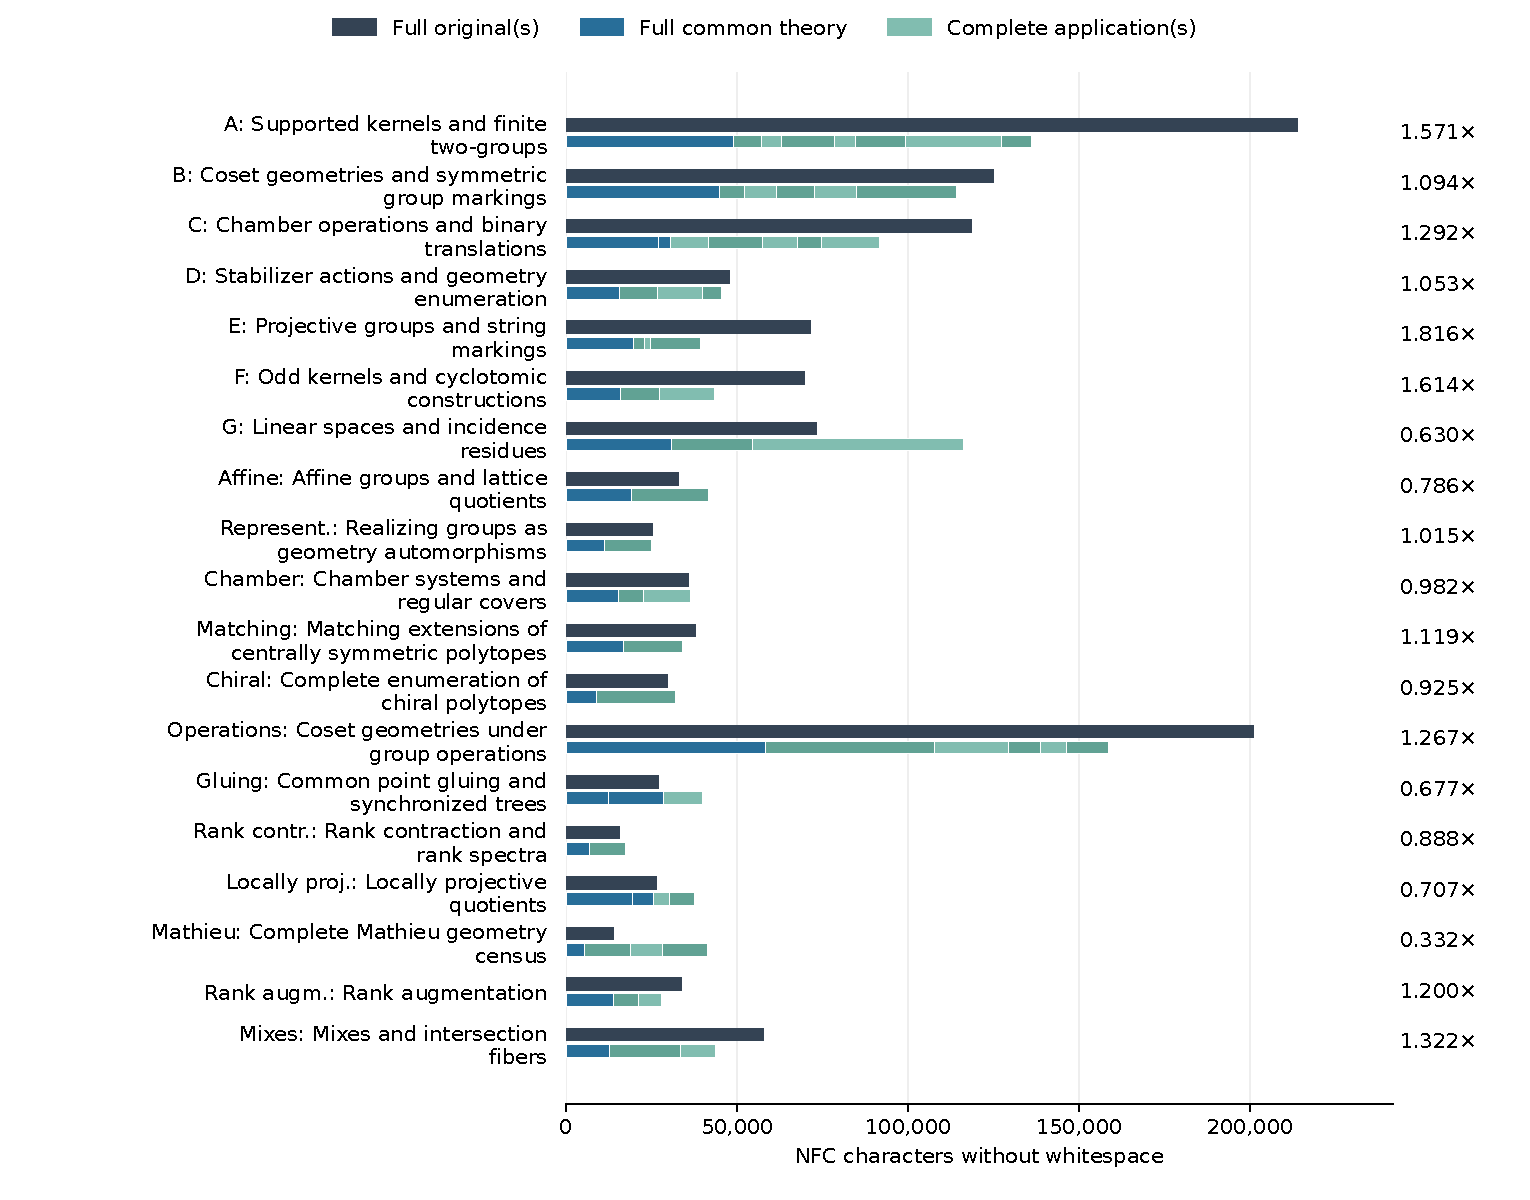
\includegraphics[width=\linewidth]{whole_topics.pdf}\end{center}
F now comprises two originals. Its entire seven-page common theory costs
15,876 characters and its five- and six-page applications cost 11,504 and
15,894. Thus $69{,}825/43{,}274=1.613555\ldots$.
The eighteen other topics retain their previous written costs. This is a
measurement of the present proofs' written length, not of minimum proof
complexity or originality.
\newpage
\textbf{Each complete application after acquisition.}
The entire common theory and all required dependencies have already been
acquired. Optional validation is not a mathematical prerequisite. Every
application, companion and reference is still charged.
\begin{center}\fontsize{8.5}{10.2}\selectfont\setlength{\tabcolsep}{5pt}
\renewcommand{\arraystretch}{1.10}\begin{tabular}{lllrrr}\toprule
Topic & Original & Application & Source cost & Application cost & Conditional\\\midrule
A & L032 & A1 & 16,558 & 8,212 & 2.016 \\
A & L034 & A2 & 21,433 & 5,784 & 3.706 \\
A & F016 & A3 & 43,983 & 15,419 & 2.853 \\
A & F013 & A4 & 25,562 & 6,224 & 4.107 \\
A & L035 & A5 & 51,019 & 14,498 & 3.519 \\
A & N009 & A6 & 36,824 & 28,114 & 1.310 \\
A & L128 & A7 & 18,424 & 8,768 & 2.101 \\
B & N001 & B1 & 14,519 & 7,371 & 1.970 \\
B & N003 & B2 & 17,780 & 9,155 & 1.942 \\
B & N008 & B3 & 18,009 & 11,132 & 1.618 \\
B & L030 & B4 & 22,704 & 12,286 & 1.848 \\
B & L040 & B5 & 51,894 & 29,321 & 1.770 \\
C & L088 & C1 & 13,166 & 11,311 & 1.164 \\
C & N013 & C2 & 27,361 & 15,815 & 1.730 \\
C & L108 & C3 & 12,849 & 10,075 & 1.275 \\
C & F014 & C4 & 20,577 & 6,962 & 2.956 \\
C & L068 & C5 & 44,480 & 17,085 & 2.603 \\
D & L066 & D1 & 20,916 & 10,989 & 1.903 \\
D & L074 & D2 & 20,661 & 13,367 & 1.546 \\
D & L104 & D3 & 6,317 & 5,499 & 1.149 \\
E & L083 & E1 & 20,885 & 3,002 & 6.957 \\
E & L079 & E2 & 20,908 & 1,855 & 11.271 \\
E & L021 & E3 & 29,582 & 14,656 & 2.018 \\
F & L014 & F1 & 25,574 & 11,504 & 2.223 \\
F & L007 & F2 & 44,251 & 15,894 & 2.784 \\
G & L009 & G1 & 49,891 & 23,544 & 2.119 \\
G & L092 & G2 & 23,308 & 61,663 & 0.378 \\
Affine & L012 & AF1 & 32,767 & 22,638 & 1.447 \\
Represent. & F010 & R1 & 25,348 & 13,688 & 1.852 \\
Chamber & L008 & H1 & 21,784 & 7,571 & 2.877 \\
Chamber & N016 & H2 & 14,018 & 13,683 & 1.024 \\
Matching & F015 & M1 & 37,951 & 17,168 & 2.211 \\
Chiral & L028 & CE1 & 29,599 & 23,171 & 1.277 \\
Operations & N005 & OP1 & 122,002 & 49,595 & 2.460 \\
Operations & N006 & DG2 & 56,001 & 38,479 & 1.455 \\
Operations & N007 & DG1 & 22,888 & 12,305 & 1.860 \\
Gluing & L010 & GL1 & 27,081 & 11,565 & 2.342 \\
Rank contr. & L037 & RC1 & 15,530 & 10,555 & 1.471 \\
Locally proj. & L084 & LP1 & 2,071 & 4,857 & 0.426 \\
Locally proj. & L095 & LP2 & 24,419 & 7,109 & 3.435 \\
Mathieu & L073 & MC1 & 13,736 & 35,862 & 0.383 \\
Rank augm. & L020 & RA1 & 33,604 & 14,096 & 2.384 \\
Mixes & F005 & MX1 & 57,753 & 31,077 & 1.858 \\
\bottomrule\end{tabular}\end{center}
DG2 includes all N006 companions. MC1 includes all 24 Mathieu application
pages. RA1 includes its application and counterproof; MX1 includes both
local papers. F1 and F2 use the same whole common theory. In F, all nine
programs are optional validation and none is a premise of the uniform proofs.
\newpage
\textbf{Original and application costs: first twenty-one originals.}
Dark bars show whole original manuscripts and green bars show whole
applications. The bars share one scale within each chart. The factors
assume prior acquisition of the complete common material.
\begin{center}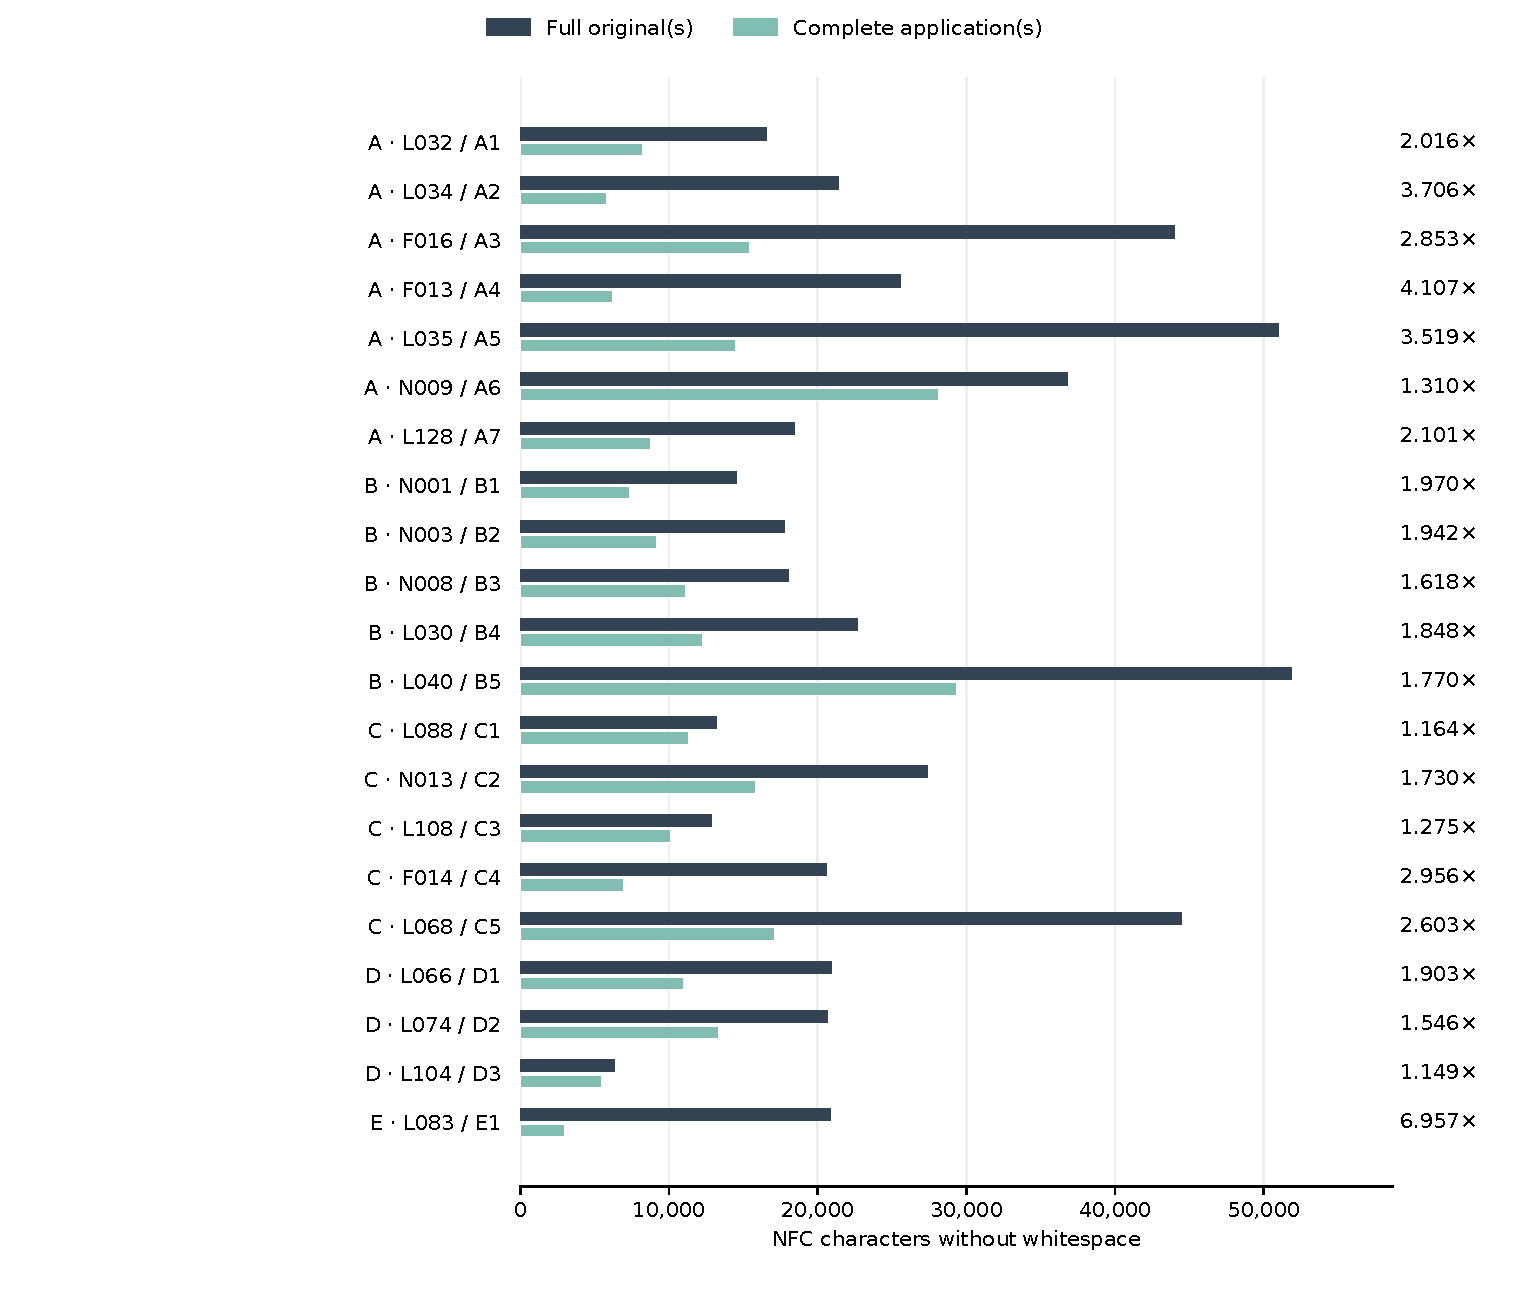
\includegraphics[width=\linewidth]{conditional_1.pdf}\end{center}
The numerical input retains the exact edition, source qualifications and
all alternative counting coordinates for each topic. F's primary coordinate
now counts raw page furniture consistently; the old selected L014 cost of
25,115 is not substituted for its current raw cost of 25,574.
\newpage
\textbf{Original and application costs: remaining twenty-two originals.}
The same complete-document convention applies. A large conditional factor
does not mean that the shared theory was free to establish.
\begin{center}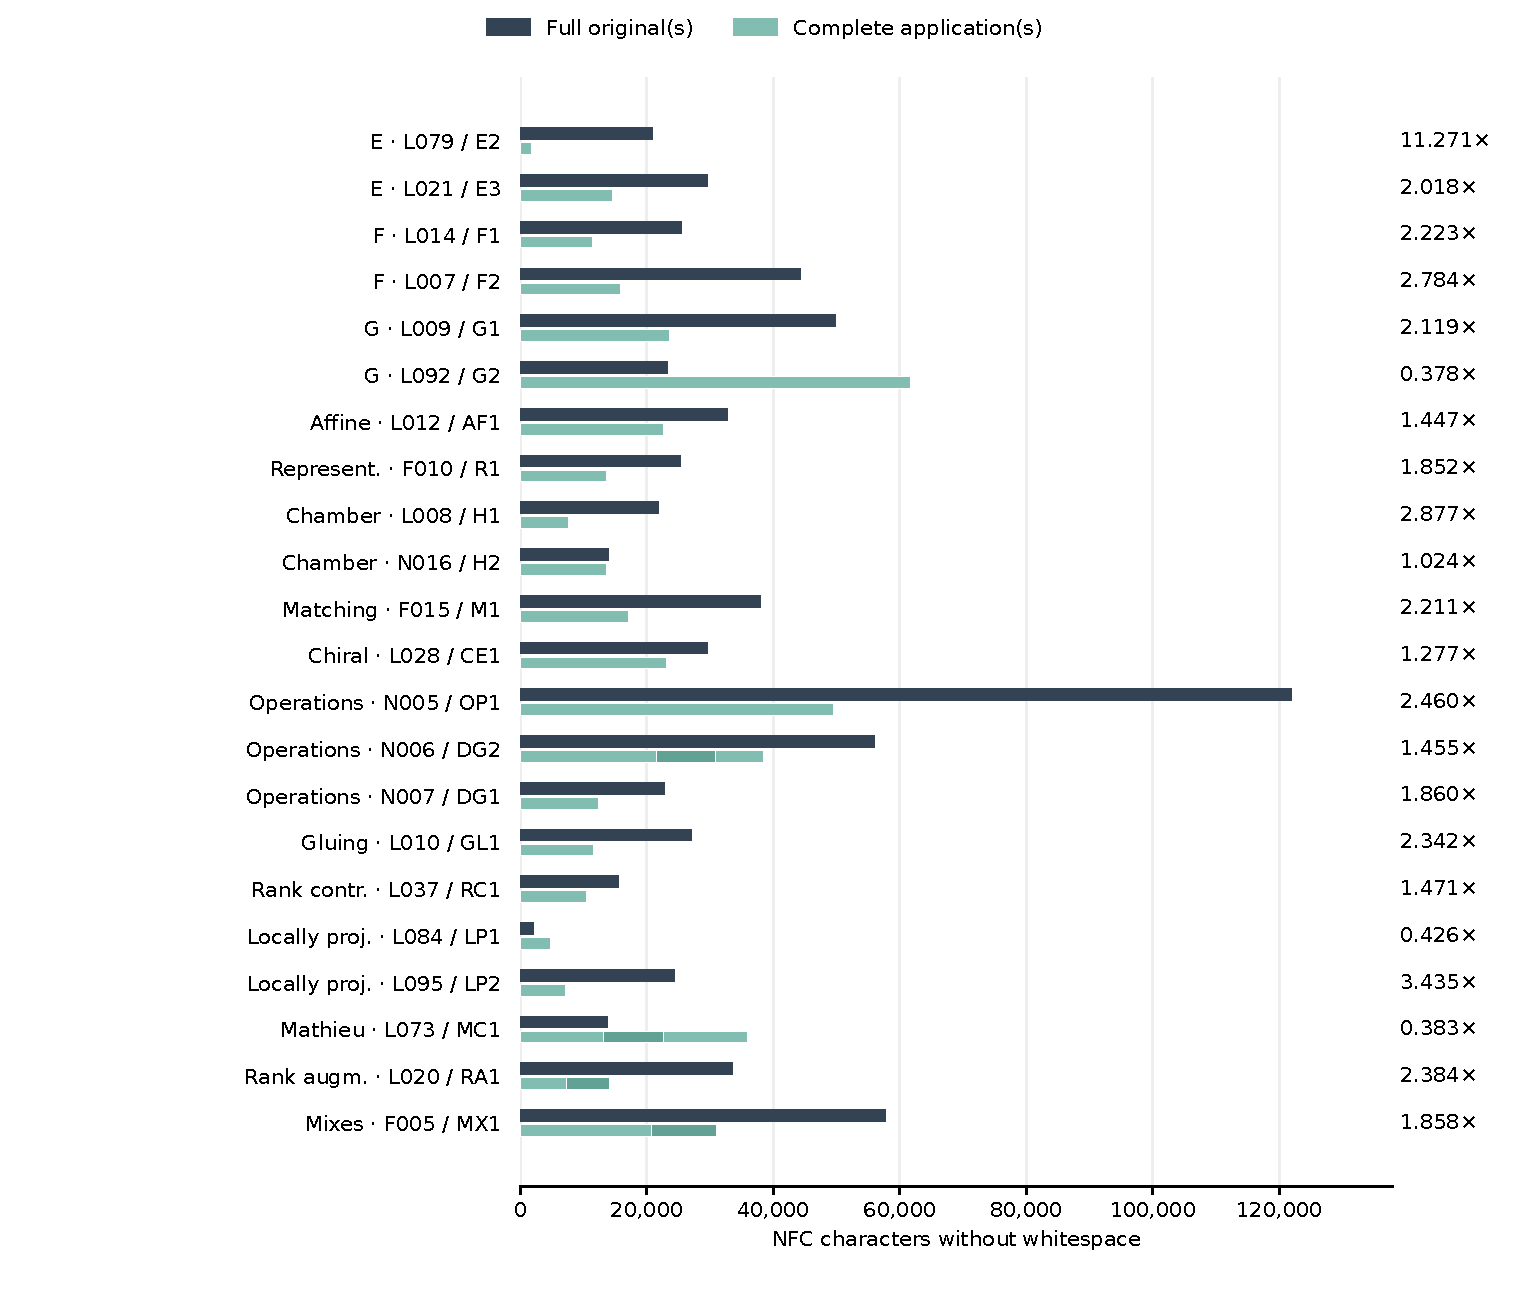
\includegraphics[width=\linewidth]{conditional_2.pdf}\end{center}
The locally projective source L084 is the complete erratum; L095 uses the
available fifteen-page arXiv edition. The Mathieu application contains the
corrected 81/431-class census and every literal source-row disposition.
L020's false third case has a corrected criterion and complete counterproof.
The Mixes paper's three final problems remain unanswered. These qualifications
remain part of the scientific admissions.
\newpage
\textbf{Program and data inventory.}
Validation must be excluded on both sides or included on both sides.
The earlier software-inclusive fractions added only our programs and are
withdrawn as compression measures. An inclusive comparison requires
\[
\frac{S+c(\text{original validation})}{U+A+c(\text{our validation})}.
\]
Original software costs are not yet established under a common inclusion
rule, so this ratio is unavailable. The following replacement costs remain
visible as inventory. Printed and raw programs are alternatives.
\begin{center}\tabsetup\begin{tabular}{lrrr}\toprule
Topic & Printed programs & Raw programs & Mandatory data\\\midrule
A & 54,210 & 52,807 & -- \\
B & 13,170 & 12,330 & -- \\
C & 20,933 & 19,937 & -- \\
D & 27,070 & 26,185 & -- \\
E & 7,565 & -- & -- \\
F & 22,466 & 21,691 & -- \\
G & 53,018 & 50,184 & -- \\
Affine & 17,250 & 16,682 & -- \\
Represent. & 9,025 & 8,310 & -- \\
Chamber & 7,677 & 6,401 & -- \\
Matching & 4,998 & 4,408 & -- \\
Chiral & 11,940 & 11,090 & -- \\
Operations & -- & 403,848 & -- \\
Gluing & 13,371 & 12,768 & -- \\
Rank contr. & 2,925 & 2,501 & -- \\
Locally proj. & 22,695 & 22,104 & 28,574 \\
Mathieu & 31,244 & 30,489 & 48,686 \\
Rank augm. & 10,866 & 9,998 & -- \\
Mixes & 16,025 & 14,608 & -- \\
\bottomrule\end{tabular}\end{center}
E additionally retains 5,173 characters of optional printed validation,
separate from its 7,565-character required program. F's printed and raw
entries both represent all nine optional validation files; they are not
additional to each other. Operations' whole raw inventory includes both
required decoding programs. Its separately inventoried external data uses
byte units, which are not added to these character costs.

\textbf{Mathematical role.} A program, certificate or data file needed to
establish a theorem remains required evidence. A manuscript-length factor
does not measure the complete cost of an executable proof when such
premises lie outside the manuscript. Missing source software, full external
proofs and graphical information retain unknown costs. Partial Lean
certificates do not establish full formalization of the source theorems.

\textbf{Embedded listings.} Separate validation is excluded from both
manuscript operands. F's two original papers and three replacement papers
were checked for embedded validation listings and contain none. This
specific check has not yet been completed for all older topics, so their
unchanged complete-manuscript figures are not universally described as
program-free comparisons.

\textbf{Evidence.} Exact integers, rational comparisons, cost inventories
and document boundaries are supplied in the accompanying JSON and CSV
files. This overview adds no proof, conjecture answer or formal declaration.
Distinct review of the consolidation is required before publication.
\end{document}
